\begin{figure}[ht]
\centering

\begin{subfigure}{0.45\textwidth}
\centering
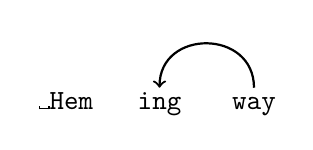
\begin{tikzpicture}[baseline, every node/.style={text height=1ex, text depth=.25ex}, node distance=1.2cm]
\node (1) {\texttt{␣Hem}};
\node (2) [right of=1] {\texttt{ing}};
\node (3) [right of=2] {\texttt{way}};
\draw[->, thick] (3.north) to[out=90,in=90,looseness=1.6] (2.north);
\end{tikzpicture}
\caption{in-boundary}
\end{subfigure}
\hfill
\begin{subfigure}{0.45\textwidth}
\centering
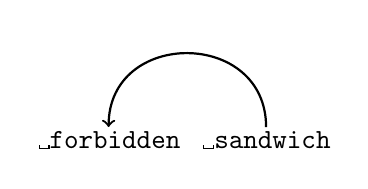
\begin{tikzpicture}[baseline, every node/.style={text height=1ex, text depth=.25ex}, node distance=2cm]
\node (1) {\texttt{␣forbidden}};
\node (2) [right of=1] {\texttt{␣sandwich}};
\draw[->, thick] (2.north) to[out=90,in=90,looseness=1.6] (1.north);
\end{tikzpicture}
\caption{out-boundary}
\end{subfigure}

\caption[Boundary condition examples]{Examples of each condition in GPT-2: in-boundary (left) and out-boundary (right). Arrows denote attention from a source token to a target token.}
\label{fig:boundary_example}
\end{figure}
